\subsection{GPU ISA Encoding Solver and Assembler}

The ISA encoding information which is necessary to build an assembler is not released by GPU vendors.
Previous third-party work to build GPU assemblers~\cite{decuda,asfermi,maxas} also
involves cracking GPU ISA encodings, whereas no cracking process is explicitly reported.
Our solver is proposed to make cracking GPU ISA encodings simple, automatic, and portable to future GPUs.

Operands could be registers (e.g. {\tt R5}),
global memory (e.g. {\tt [R6+0x20]}), constant memory (e.g. {\tt C[0x2][0x40]}), shared memory (e.g. {\tt [0x50]}), immediate values (e.g. {\tt 0x9} and {\tt1.5}), or predicate registers (e.g. {\tt P3})~\cite{ptx2015isa}.
We observe that an operand name always includes a number, thus an operand can be inferred by its name.
Since a number's encoding can be literally explained, the operand encoding is relatively easy to recognize.
For example, the register operand {\tt R5} can be inferred from $101$ in binary format, while the immediate value {\tt 0x9} is $1001$. 
%Besides, the fixed lengths of these fields allow us to determine their positions \jled{and lengths, don't need to specify lengths here.} relatively easily and hence to encode them. 
The encodings of opcodes and modifiers are mnemonic symbols which can not be literally explained,
a heuristic algorithm is designed to crack the positions of them.
Besides, Modifiers are instruction-specific, modifiers in the same type may have different encodings for different instructions. 
As an example, masks of type-size modifier for instructions {\tt LD} and {\tt LDG} are in different binary positions. 
Hence, every instruction's modifier need to be processed independently. 


% \begin{figure}[htbp]
% \begin{center}
% 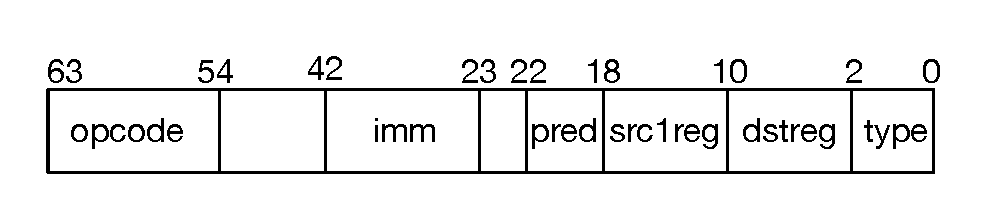
\includegraphics[scale=0.5]{imm}
%     \caption{IADD instruction encoding format}
% \label{fig:imm}
% \end{center}
% \end{figure}

% Figure~\ref{fig:imm} shows encoding format of {\tt IADD} instruction with {\tt opcode}, {\tt operand}, and {\tt modifier} fields.
%We express a native assembly instruction in a struct variable $inst$, which is the input of our solver.
%In this way, we generate real assembly instruction and their 64-bit encoding, which is the input of solver algorithm.
%We disassmble libcublas.so to generate instruction and their corresponing 64-bit encodings. There are $1537123$ different encodings of cublas 7.0 library in total.



\subsubsection{Opcode and Modifier Solvers}
% \subsubsection{Opcode Encoding Solver}
We design a heuristic algorithm (Algorithm~\ref{algo:opcode}) to crack {\tt opcode} encodings by detecting their bit positions.
Opcode solver takes $N$ diassembly instructions generated from PTX samples as the input and outputs all opcode positions as $opBits$.
Each diassembly instruction $inst$ integrates its 64-bit binary code, name, operand types, and operand values as a structure.
Take the $IADD$ instruction in Equation~\ref{eq:iadd} for example, its binary code is $0x4800000000201c03$, name is $IADD$, operand types is represented a string ``RRR'', and operand values are represented as a tuple $\{ 0,2,0 \}$.
By flipping the 64 bits one-by-one, we determine whether each bit belongs to opcode.
Each flip generates a new binary code $\widehat{enc}$ which is disassembled by nvdisasm to a new instruction $\widehat{inst}$.
If $\widehat{inst}$ is valid and its instruction name is changed, this bit is in opcode field.

% is to write intermediate codes based on NVIDIA PTX syntax, and generate encoding by NVIDIA toolchain.
% Subsequently, the opcodes can be achieved by stripping out operand masks, and
% flags can be found by stripping out both opcodes and operand masks.
% However, the uncompleteness of NVIDIA document hinders us from finding out all the opcodes and instruction modifiers. 
% Another feasible way is to find the bit positions which represents opcode, then
% enumerate all the possible binary combinations after stripping out operand masks as Algorithm~\ref{algo:opcode} shows.

From our results of NVIDIA Tesla K20m, we find that the highest $10$ bits and the lowest $2$ bits represent opcode on GPU Kepler architecture.
This algorithm narrows the opcode search space from $64$ to $12$ bits with an acceptable running time of $O(64N)$, where $N$ is the number of disassembly input generated from PTX samples ($N$ is around $2300$ in our experiment). %\jli{add sample number}.
We only enumerate possible opcodes in the pruned $12$ bits and identify all valid ones.

% Thus, we only enumerate these opcode bits which generate an acceptable search space. Finally, we find 
% the minimal opcode without any flags. 
A modifier defines a specific behavior of an instruction. 
For example, {\tt LD} instruction has type-size modifiers, such as {\tt .u8}, {\tt .s8}, {\tt .u16}, {\tt .32}, {\tt .64} and {\tt .128}, and cache operation modifiers, such as {\tt .CS}(cache streaming) and {\tt .CG} (cache at global level). 
%A modifier is more complicated to detect because its position spans across all the remaining bits and an instruction may have more than one kinds of modifiers. 
We use similar solver by flipping all these bits to observe whether its instruction
modifier. The modifier difference is checked per opcode. %that the algorithm is done per opcode name.
%The algorithm is similar to Algorithm~\ref{algo:opcode}.

\begin{algorithm}[htbp]
      \caption{Opcode Solver}\label{algo:opcode}
      {\small
      \begin{algorithmic}[1]
      \State \textbf {Input:} instSet, $N$ diassembly instructions generated from PTX samples
      \State \textbf {Onput:} opBits, opcode positions in the 64-bit encoding
      \For {$i \gets 0, \dots, N-1$}
	  %\LineComment {fetch an instruction from generated database \jled{what's the database?}}
      %\State \For i in instMap
      \LineComment {$inst$ structure: \{enc64, name, oprdType, oprd\}}
      \State $inst$ = instSet[i]
      %\State $inst \gets instMap[i]$
      \LineComment {the 64-bit encoding of the instruction}
      \State $enc \gets$ inst.enc64
	\LineComment {check each bit of $enc$ for opcode}
      \For {$j \gets 0, \dots, 63$}
      %\LineComment {if bit $j$ not operand bit and its value is 0} % \jled{what about enc[j]!=0? No need to check if it is opcode?}}
      %\If {notOprd($enc[j]$) and $enc[j] = 0$}
      \LineComment {flip the $j^{th}$ bit of the encoding}
      \State $\widehat{enc}$ = xorAt($enc, j$)
	  \LineComment {disassemble new encoding $\widehat{enc}$}
      \State $\widehat{inst}$={\tt nvdisasm}($\widehat{enc}$)
	  \LineComment {bit-$j$ is in the opcode field if $\widehat{inst}$ is a different instruction.}
      \If { isvalid($\widehat{inst}$) and inst$.name\neq \widehat{inst}.name$}
      \State put($j$, $opBits$)
      %\EndIf
      \EndIf
      \EndFor
      \EndFor
      \State \textbf{Return} opBits 
  \end{algorithmic}
  }
\end{algorithm}

% \begin{algorithm}[htbp]
%       \caption{Opcode Solver}\label{algo:opcode}
%       {\small
%       \begin{algorithmic}[1]
%       \State \textbf {Input:} diassembly generated by PTX samples
%       \State \textbf {Onput:} Opcodes' positions in 64-bit encoding
%       \For {$i \gets 0, N$}
%         %\LineComment {fetch an instruction from generated database \jled{what's the database?}}
%       %\State \For i in instMap
%       \LineComment {structure of inst\{ op, enc64, oprdType, oprd\}}
%       \State inst = instParser(line[i])
%       %\State $inst \gets instMap[i]$
%       \LineComment {the 64-bit encoding of the instruction}
%       \State $enc \gets inst.enc64$
%         \LineComment {check each bit of $enc$ for opcode}
%       \For {$j \gets 0, 63$}
%       %\LineComment {if bit $j$ not operand bit and its value is 0} % \jled{what about enc[j]!=0? No need to check if it is opcode?}}
%       %\If {notOprd($enc[j]$) and $enc[j] = 0$}
%       \LineComment {flip $jth$ bit of 64-bit encoding}
%       \State nEnc = xorAt($enc, j$)
%         \LineComment {disassemble new encoding nEnc}
%       \State nInst=nvdisasm(nEnc)
%         \LineComment {bit $j$ belongs to an opcode if it is changed }
%       \If { isvalid(nInst) and $nInst.op\neq inst.op$}
%       \State put($j$, $opBits$)
%       %\EndIf
%       \EndIf
%       \EndFor
%       \EndFor
%       \State \textbf{Return} opBits %\jled{All instructions' opcodes are stored in opBits?}
%   \end{algorithmic}
%   }
% \end{algorithm}

\subsubsection{Operand Solver}
% \subsubsection{Operand Position Solver}
Algorithm~\ref{algo:operand} shows our algorithm to crack operand encodings.
Since each instruction may have different numbers and types of operands, we identify operand positions a tuple of its name and operand type. 
The operand types of an instruction are represented as a string.
For example, oprdType of the instruction {\tt IADD} R1, R2, C[0x0][0x40] is ``RRC'' and oprdType of {\tt IADD} R1, R2, 0x8 is ``RRI'', where R, C and I represents registers, constant memory and immediates respectively.
For each instruction with the known opcode, we flip each undetermined bit to get a new instruction $\widehat{inst}$.
Comparing $inst$ with $\widehat{inst}$ using a simple function ``whichChange'' we confirm which operand value is changed by its position if any, that is $p>0$.
Otherwise, this bit doesn't belong to the operand field.
Then the visited dictionary is marked as 1.
Algorithm~\ref{algo:operand}'s time complexity is $O(52N)$, where $N$ is the number of diassembly instructions with different opcodes.

\begin{algorithm}[htbp]
      \caption{Operand Solver}\label{algo:operand}
      {\small
      \begin{algorithmic}[1]
      \State \textbf {Input:} instSet, $N$ diassembly instructions with different opcodes
      \State \textbf {Onput:} pos, operand positions for each opcode, a 2D array.
      \State {visited=\{\}}
      \Comment {A dictionary to record the visited information of an operand bit, key:$\langle$name, oprdType$\rangle$}
      \For {$i \gets 0, \dots, N$}
	  %\LineComment {fetch an instruction from generated database \jled{what's the database?}}
      \LineComment {$inst$ structure: \{enc64, name, oprdType, oprd\}}
      \State inst = instSet[i]
      %\State $inst \gets instMap[i]$
      %\State $enc \gets inst.enc64$
	\LineComment {check the rest bits of $enc$ for operand by excluding opcode bits}
      \For {$j \gets 2, \dots, 53$}
      %\LineComment {if bit $j$ not operand bit and its value is 0} % \jled{what about enc[j]!=0? No need to check if it is opcode?}}
      %\If {notOprd($enc[j]$) and $enc[j] = 0$}
      \LineComment {flip $j^{th}$ bit of enc}
      \State $\widehat{enc}$ = xorAt($enc, j$)
	  \LineComment {disassemble new encoding $\widehat{enc}$}
      \State $\widehat{inst}$={\tt nvdisasm}($\widehat{enc}$)
	\LineComment {If bit-$j$ is an operand bit, return the operand position.}
      \State p = whichChange($inst$,$\widehat{inst}$)
      \If {$p > 0$}
      \State put(j, pos[$\langle$inst.name,inst.oprdType$\rangle$][p])
      \LineComment{Mark $\langle$name, oprdType$\rangle$ as visited}
      \State visited[$\langle$inst.name,inst.oprdType$\rangle$] = 1
      \EndIf
      \EndFor
      \EndFor
      \State \textbf{Return} pos 
  \end{algorithmic}
  }
\end{algorithm}


% \begin{algorithm}[htbp]
%       \caption{Operand Solver}\label{algo:operand}
%       {\small
%       \begin{algorithmic}[1]
%       \State \textbf {Input:} diassembly with all the opcodes generated by opcode solver
%       \State \textbf {Onput:} Operand positions for each opcode
%       \LineComment {A hash table to check if an operand bit position is visited, key:<opcode, operandType> }
%       \State {visited=\{\}}
%       \For {$i \gets 0, N$}
%         %\LineComment {fetch an instruction from generated database \jled{what's the database?}}
%       \LineComment {structure of inst\{ op, enc64, oprdType, oprd\}}
%       \State inst = instParser(line[i])
%       %\State $inst \gets instMap[i]$
%       %\State $enc \gets inst.enc64$
%         \LineComment {check each bit of $enc$ for opcode}
%       \For {$j \gets 0, 63$}
%       %\LineComment {if bit $j$ not operand bit and its value is 0} % \jled{what about enc[j]!=0? No need to check if it is opcode?}}
%       %\If {notOprd($enc[j]$) and $enc[j] = 0$}
%       \LineComment {flip $jth$ bit of enc by xor}
%       \State nEnc = xorAt($enc, j$)
%         \LineComment {disassemble new encoding nEnc}
%       \State nInst=nvdisasm(nEnc)
%         \LineComment {If bit $j$ is an operand bit, return the order of operand}
%       \If {ith = whichChange(origin,new) > 0}
%       \State pos[origin.op][origin.oprdType][ith].append(j)
%       \LineComment{Mark <op, oprdType> is visited}
%       \State visited[origin.op][origin.oprdType] = 1
%       \EndIf
%       \EndFor
%       \EndFor
%       \State \textbf{Return} pos 
%   \end{algorithmic}
%   }
% \end{algorithm}


%\subsubsection{Modifier Solver}


%Algorithm~\ref{algo:int_solver} shows the pseudocode for immediate operand decoding process. 
%The basic idea is matching the binary encoding of an operand in $64$-bit instruction encoding and finding
%position until the position is unique. The input instructions are from disassembly codes.
%First, we randomly pick up an instruction that has the field we want to probe and represent the field in binary by its 
%name. Second, we match the operand binary in $64$-bit instruction encoding and find possible positions. Third, we 
%intersect current candidates with previous ones. %If the number of candidates is $1$, we find the position. 
%The unique position is found when the number of candidates is $1$.
%Otherwise, 
%we set the current candidate to the previous one and randomly pick up next instruction to repeat the procedure.
%Other operand types such as register operand can use similar routine by matching the corresponding operand binary.
%Once the operand position is found, we need to probe or verify the length of the operand encoding. Some are easy to be
%deduced. For example, each thread can use at most $256=2^{8}$ registers, we could predict the length of register 
%operand mask to be $8$.
%However, other operand types like immediate $0x48$ or subscript of constant memory $C[0x2][0x05]$, are more complicated 
%to predict. Our solution is to set the bits from the position bit by bit to check whether the operand value grows
%as expected. For instance, by using Algorithm~\ref{algo:int_solver}, we find out that the immediate operand position 
%of {\tt IADD RX, RY, 0ximm} (the RX and RY are arbitrary register operands, 0ximm is an immediate operand) is at bit $23$ 
%as shown in Figure~\ref{fig:imm}. As specified in~\cite{cuda2015programming}, NVIDIA GPU uses little-endian 
%representation, then we set the bits higher than the $23$ to $1$ bit by bit, and observe the disassembled code. 
%Immediate value increases continuely until reaches value {\tt 0x7ffff}, which means that $41\sim23$ is for integer 
%immediate.%No {\tt fffff} immediate was got even if we set bit $42$ to be $1$.  


